%!TEX root = main.tex

\begin{figure*}[htbp]
	\centering
	\newcommand\myheight{0.162}
	\subfloat[] {
		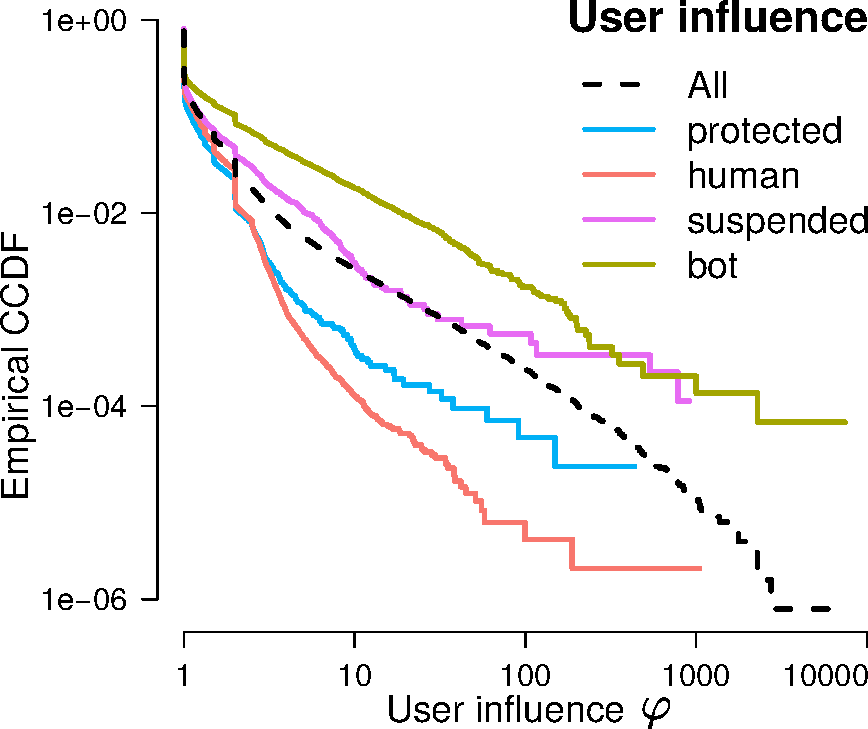
\includegraphics[height=\myheight\textheight]{2017-11-13-CCDF-influence-4-populations}
		\label{subfig:user-infl-CCDF}
	}
	\subfloat[] {
		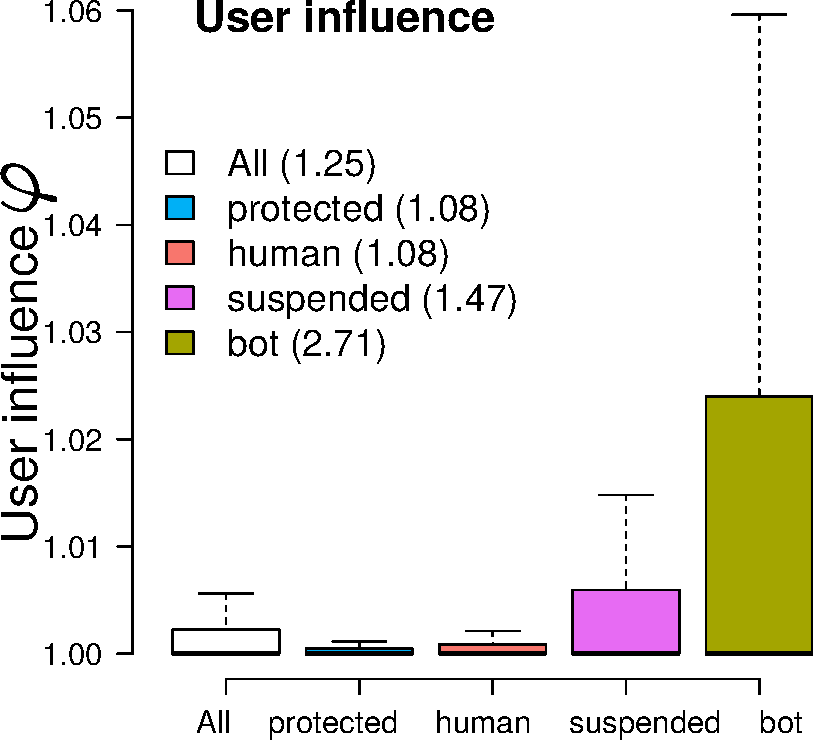
\includegraphics[height=\myheight\textheight]{2017-11-13-boxplot-influence-4-populations}
		\label{subfig:user-infl-boxplots}
	}
	\subfloat[] {
		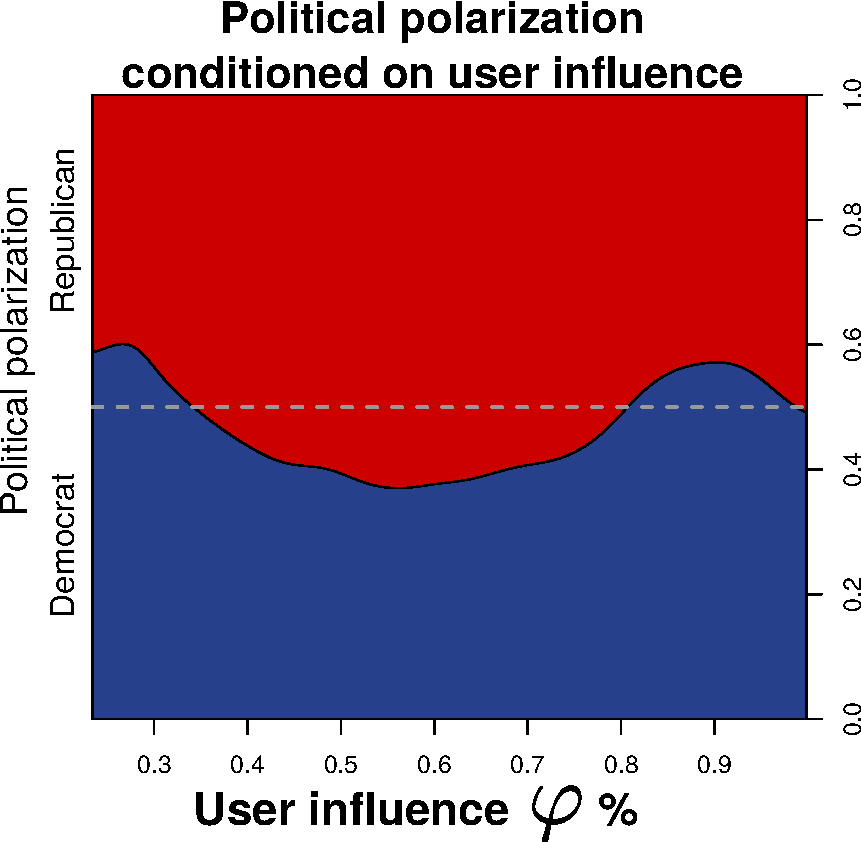
\includegraphics[height=\myheight\textheight]{influence_conditional_density}
		\label{subfig:polarization-conditioned-user-infl}
	}
	\subfloat[] {
		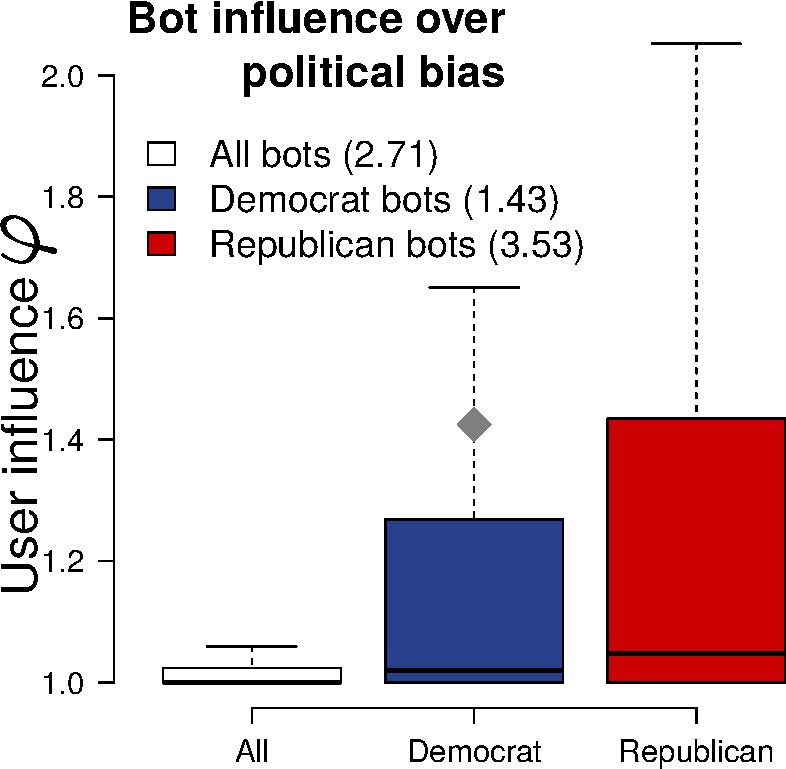
\includegraphics[height=\myheight\textheight]{BOTS_boxplot-influence-vs-political-bias}
		\label{subfig:bot-influence}
	}
	\caption{ 
		Profiling influence, and linking to botness and political behavior.
		\textbf{(a)(b)} User influence $\varphi(u)$ for the reference populations, shown as log-log CCDF plot (a) and boxplots (b).
%		The influence in each of the four reference populations is long-tail distributed.
%		\textbf{(b)} Boxplot of user influence for the four bot populations -- 
		\textbf{(c)} Probability distribution of polarization, conditional on $\varphi(u) \%$.
		\textbf{(d)} Boxplots of user influence for the pro-Democrat and pro-Republican \Bot users.
		% (dashed line), and for the democrat and republican polarized populations (blue and red lines respectively).
		%\TODO{MAR}{Message in text: republican bots are more engaged than democrat bots.}
		Numbers in parenthesis show mean values.
	}
%	\label{fig:holdout-ll}
%	\captionmoveup
\end{figure*}